\chapter{Architecture}

Dans ce chapitre, on ne fait pas toujours la distinction entre un composant (au sens de composant SlipStream)
et une VM (qui est un composant déployé).
Il faut toutefois rappeler qu'un composant peut être déployé plusieurs fois.

De la même manière, nous utilisons le mot \og{} composant \fg{} pour parler d'un composant SlipStream
et d'un composant (logiciel) de MicroScope.
Le contexte devrait permettre d'éviter toute ambiguïté.

\section{Vue d'ensemble}

La vue d'ensemble de l'architecture est présentée dans la~\autoref{fig:architecture}.
Il y 5 composants Nuvla et
1 VM permanente déployée sur le cloud \cloudInstance{ifb-prabi-girofle}.

\begin{figure}[htp]
    \centering
    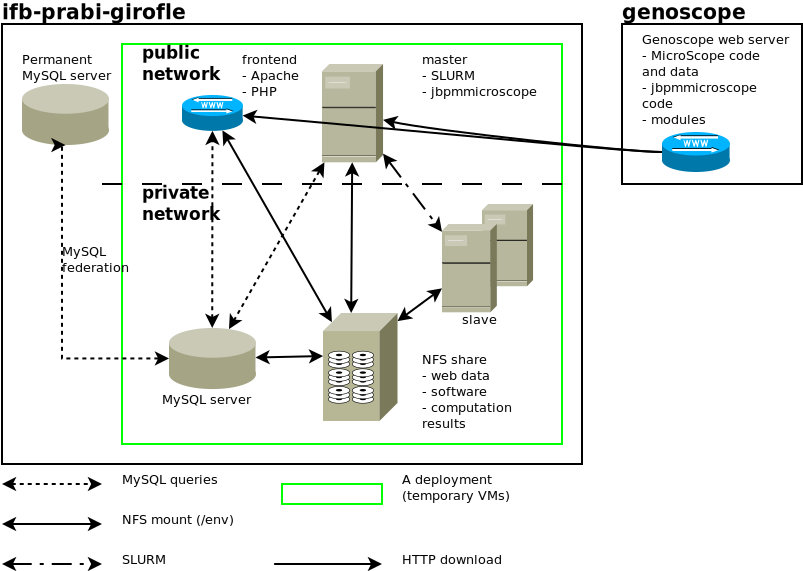
\includegraphics[width=\linewidth]{../Logical_Architecture}
    \caption{Schéma de l'architecture de MicroCloud.}
    \label{fig:architecture}
\end{figure}

Un des buts est de mimer ce qui est fait au Genoscope
c'est-à-dire que:
\begin{enumerate}
    \item Les différents composants (serveur web, serveur de BD, etc.) tournent sur des machines séparées.
    \item Les calculs tournent sur des machines séparées: l'architecture contient donc un cluster (basé sur SLURM).
\end{enumerate}
Une des seules différences est que le serveur \component{jbpmmicroscope} tourne
sur la machine frontale du cluster.

Lors du déploiement, les VM téléchargent des fichiers (code et données) depuis le serveur web du Genoscope.
Ces fichiers sont crées par le module \micWEBdeployVer{} (voir~\autoref{chap:micwebdeploy}).
Le gros du travail du travail est fait dans les scripts de la phase Deployment (script \script{04\_Deployment.sh} de chaque composant SlipStream).
Ceci a été fait pour simplifier les scripts d'installation et ne pas fixer les versions de MicroScope à ces étapes.

Il y a 2 serveurs de bases de données dans MicroCloud\todo{Renvoyer à section choix techniques.}:
\begin{itemize}
    \item Un serveur MySQL installé via Docker dans la VM MySQL.
    \item Un serveur MySQL sur la VM permanente.
\end{itemize}

\section {Installation et déploiement des VM}

Le code des composants Nuvla est dans le dépôt \project{biosphere-microcloud}.
Il y a un dossier par composant et un fichier \filename{README.md} dans chaque dossier qui explique des détails.
Les principes du déploiement sont décrits sur le wiki du projet (voir la page
\href{https://intranet.genoscope.cns.fr/agc/redmine/projects/microcloud/wiki/Principes_de_fonctionnement_du_cloud_IFB}
{[[Principes de fonctionnement du cloud IFB]]}
en particulier la section
\href{https://intranet.genoscope.cns.fr/agc/redmine/projects/microcloud/wiki/Principes_de_fonctionnement_du_cloud_IFB#Utilisation-de-deacutepocircts-git-pour-le-code}
{[[Utilisation de dépôts git pour le code]]}
).

Les sections suivantes présentent quelques détails sur les VM:
\begin{itemize}
    \item \SScomponent{frontend} voir section \ref{frontend}
    \item \SScomponent{mysql} voir section \ref{mysql}
    \item VM permanente voir section \ref{VMpermanente}
    \item \SScomponent{master} et \SScomponent{slave} voir section \ref{master&slave}
    \item \SScomponent{nfsserver} voir section \ref{nfsserver}
\end{itemize}
Comme expliqué, le code de chaque composant est dans un dossier éponyme dans le dépôt biosphere-microcloud.
Dans les sections sus-citées, le nom des scripts est relatif à ce dossier (sauf mention contraire).

\subsection {Composant \SScomponent{frontend}}\label{frontend}

La composant \SScomponent{frontend} permet de déployer la partie web de la plateforme MicroScope.
L'image de base est une image CentOS 7.

\paragraph*{Configuration}

Le script \script{04\_Deployment.sh} réalise un certain nombre d'opérations avant l'installation de MicroScope:
\begin{itemize}
    \item Configuration de \component{Apache} (génération d'un certificat SSL)
          et \component{PHP} (variables \variable{memory\_limit}, \variable{max\_execution\_time},  \variable{max\_input\_time})
          nécessaires pour MicroScope.
    \item Configuration d'un alias du composant \SScomponent{mysql} sous le nom \hostname{mysqlagcdb.genoscope.cns.fr}
          (ceci a été fait pour ne pas avoir à modifier la configuration de MicroScope).
    \item Configuration de \component{phpMyAdmin}.
    \item Montage du répertoire partagé.
\end{itemize}

\begin{mycolorbox}
    La VM \SScomponent{frontend} utilise un client mariaDB (et non pas MySQL du fait de conflits existants entre le dépôt remi-php71 installé et le dépôt IUS qui fournit le client MySQL).
\end{mycolorbox}

\paragraph*{Installation de MicroScope}

Le script \script{install\_microscope.sh} réalise l'installation de MicroScope:
\begin{itemize}
    \item Création de l'utilisateur MySQL \user{agc} (avec le mot de passe habituel).
    \item Création des bases de données nécessaires à l'instance et copie des données minimales.
          Les tables nécessaires à l'installation de MicroScope (hors bases des banques qui sont dans la VM permanente)
          sont listées dans la page wiki           \href{https://intranet.genoscope.cns.fr/agc/redmine/projects/microcloud/wiki/Tables_necessaires_a_installation}{[[Tables nécessaires à l'installation]]}.
    \item Copie du code web dans le répertoire \variable{DOCUMENT\_ROOT} de la VM (\path{/var/www/html/})
          et des scripts dans \path{/var/www/binphp/} (variable \variable{BIN} dans la configuration de MicroScope).
\end{itemize}

\paragraph*{Import des données de l'organisme \theOrg{}}

Les données de \theOid{} sont copiées avec le script \script{import\_Oid.sh}.

\begin{mycolorbox}
    Si lors de la connexion au serveur web le message d'erreur \textbf{256} s'affiche, cela signifie qu'il n'y a pas d'organisme en base.
    De ce fait, la plupart des onglets ainsi que le formulaire d'authentification sont inaccessibles.
    Ceci ne doit pas arriver si le déploiement se passe bien car on on copie les données d'un organisme.
\end{mycolorbox}

\paragraph*{Création des liens FEDERATED}

Les liens FEDERATED vers la VM permanente (qui permettent d'accéder aux base représentant les banques) sont crées
dans le script \script{create\_federated\_links.sh}.
Le script crée automatique un lien avec toutes les BD présentes sur la VM permanente sauf les BD système (\DB{mysql}, \DB{information\_schema}, \DB{performance\_schema}, \DB{sys})
et celles liées à \component{phpMyAdmin}.

\subsection {Composant \SScomponent{mysql}}\label{mysql}

Le composant \SScomponent{mysql} est le serveur de base de données de l'instance.
L'image de base est une image CentOS 7.

Comme cette VM se trouve sur le réseau privé, il faut passer par la VM frontend pour se connecter à la VM mysql:
\begin{lstlisting}[style=bash]
ssh -A centos@${IP_mysql} -J centos@${IP_frontend}
\end{lstlisting}

\paragraph*{Installation de MySQL}

Le serveur MySQL est installé via Docker.
Si le serveur ne répond pas, il faut aller voir si le docker n'a pas planté (cela arrive pour des requêtes SQL trop gourmandes en RAM).
Pour relancer le docker :
\begin{lstlisting}[style=bash]
sudo su
docker ps -a
docker start ${ID_container}
\end{lstlisting}

\paragraph*{Installation des fonctions UDF de MicroScope}

Les fonctions UDF nécessaires à MicroScope (\component{lib\_mysqludf\_sequtils})
sont téléchargées depuis le Genoscope et
sont installées dans le docker.

\begin{mycolorbox}
    Contrairement à la plupart des autres composants, la version des fonctions UDF utilisée
    est fixée dans les scripts (\micUDFVersion) et n'est pas gérée par \micWEBdeployVer{} (voir~\autoref{chap:micwebdeploy}).
    Ceci est lié au fait que c'est le composant qui a été développé en premier
    et que \component{lib\_mysqludf\_sequtils} évolue peu.
\end{mycolorbox}

\subsection {VM permanente}\label{VMpermanente}

La procédure d'installation est dans le fichier \textbf{Installation.md} du répertoire \textbf{/root}. La VM permanente sert au stockage des données des banques. Nous avons utilisé \textbf{rsync} pour l'import des données dans le serveur MySQL.

Logiciels installés : serveur MySQL, rsync, phpMyAdmin (installé mais non configuré).

Pour se connecter :
\begin{lstlisting}[style=bash]
ssh root@134.214.33.214
\end{lstlisting}

\paragraph*{Création des BD et copie des données}

Le serveur MySQL contient les schémas des banques et les données nécessaires pour les tests (nous avons testés les onglets \textbf{Genome Browser}, \textbf{Identical Gene Names}):
\begin{itemize}
    \item les schéma des bases \DB{ANTISMASHDB}, \DB{CARDDB}, \DB{COGDB}, \DB{EGGNOGDB}, \DB{ENZYMEDB}, \DB{ESSDB}, \DB{FIGFAMDB}, \DB{INTERPRODATADB},
          \DB{KEGGDB}, \DB{RHEADB}, \DB{TAXONOMYDB}, \DB{TIGRFAMDB}, \DB{UNIFIREDB}, \DB{UNIPROTKBDB}, \DB{VIRULENCEDB}, \DB{microcyc}\footnote{Je pense cette base n'est pas nécessaire à l'heure actuelle (MD).}
          et \DB{DBWORKFLOW}.
    \item une partie des données de la base \DB{UNIPROTKBDB} pour les tests.
    \item les données de \DB{DBWORKFLOW}.
    \item les données de l'organisme \theOrg{} (taxon id \theTaxID{}) dans la base \DB{TAXONOMYDB}.
\end{itemize}

Le script \script{microscopeDBschema.py} du module MicroCloud a été utilisé pour créer les schémas.

Pour se connecter au serveur MySQL :
\begin{lstlisting}[style=bash]
mysql -p{MOT_DE_PASSE_SERVEUR_MYSQL_VM_PERMANENTE}
\end{lstlisting}

\subsection{Compoants \SScomponent{master} et \SScomponent{slave}} \label{master&slave}

\todo[inline]{Ajouter les notes sur jbpmmicroscope ici ? Notes sur conda et l'installation des modules ? Plutôt dans la partie choix techniques.}

Ces 2 composants permettent de créer un cluster basé sur SLURM sur lequel \component{jbpmmicroscope} soumet les jobs:
\SScomponent{master} est la frontale et \SScomponent{slave} est un nœud de calcul.
Le code SlipStream est basé sur les travaux de Jonathan Lorenzo et Bryan Brancotte:
\begin{itemize}
    \item Les composants \SScomponent{master} et \SScomponent{slave} ont été copiés depuis
    l'appliance \href{https://nuv.la/module/ifb/devzone/jlorenzo/cluster/Slurm_Cluster_ubuntu18}{\SScomponent{Slurm\_Cluster\_ubuntu18}}.
          L'image de base de ces composants est une image Ubuntu 18.04.
    \item Le code d'installation de ces composants a été copié depuis le dépôt \project{biosphere-commons}
          puis modifié pour les besoins de MicroCloud\todo{Préciser çà}.
\end{itemize}
Le composant \component{slave} peut être instancié plusieurs fois (2 par défaut).
Ceci est choisi lors du déploiement (voir~\autoref{chap:deploiement}).

\paragraph*{Généralités}

Les composants \SScomponent{master} et \SScomponent{slave} montent le dossier partagé \path{/env/} (voir~\autoref{nfsserver}).
Le composant \SScomponent{slave} est peu modifié par rapport aux scripts de J. Lorenzo et B. Brancotte.
En revanche, le composant \SScomponent{master} est plus complexe car
c'est sur lui qu'on installe \component{jbpmmicroscope} (et donc \component{Tomcat})
et les logiciels partagés entre la frontale et les nœuds de calcul.

\paragraph*{Installation de \component{jbpmmicroscope}}

\component{jbpmmicroscope} et le serveur d'application \href{http://mirrors.ircam.fr/pub/apache/tomcat/tomcat-9/v9.0.31/bin/apache-tomcat-9.0.31.tar.gz}{\component{Tomcat} version 9.0.31}
sont installés par \script{install\_jbpm.sh} à partir des fichiers téléchargés depuis le Genoscope.
Le script n'est pas très compliqué.

Pour accéder à Tomcat : http://\$IP\_master.

\paragraph*{Installation de \component{pegasus-mpi-cluster}}

\component{bagsub} s'appuie sur \component{pegasus-mpi-cluster}.
Nous avons installé (\href{https://github.com/pegasus-isi/pegasus/archive/4.9.2.zip}{\component{pegasus-mpi-cluster} version 4.9.2}).
Le code téléchargé ne compile pas à cause car la librairie \component{libnuma} n'est pas installée.
Comme celle-ci n'est pas nécessaire pour les architectures non-NUMA, nous modifions les fichiers \filename{Makefile}
pour supprimer la dépendance à \component{libnuma}.

\paragraph*{Installation des modules (dont \component{bagsub})}

Chaque workflow fait appel à différents modules qu'il faut installer au préalable sur la VM master.
Le script \script{import\_modules.sh} permet d'importer les archives des différents modules nécessaires au fonctionnement des workflows (WF DIRECTON principalement).

Le script \script{import\_modules.sh} fait quelques modifications du module \component{bagsub} afin qu'il puisse être utilisé dans l'environnement fourni par la VM \SScomponent{master}:
on supprime l'option ulimit qui ne fonctionne pas en \component{dash} (le shell sous Ubuntu 18.04)
et ajoute le paramètre MCA \variable{btl\_tcp\_if\_exclude} pour exclure les interfaces réseaux \hostname{docker0} et \hostname{lo} qui peuvent engendrer des conflits lors du lancement de jobs SLURM.


\subsection{Composant \SScomponent{nfsserver}} \label{nfsserver}

Le composant \SScomponent{nfsserver} a été créé en s'inspirant du travail de Stéphane Delmotte.
Il permet de fournir un dossier partagé entre les différentes VM.
L'image de base est une image CentOS 7.

Le répertoire \path{/var/nfsshare} du serveur NFS est monté dans le répertoire \path{/env}
des composants \SScomponent{frontend}, \SScomponent{backend}, \SScomponent{master} et \SScomponent{slave}.
Le répertoire \path{/env/} se veut similaire au répertoire de même nom sur le cluster \hostname{etna}.

Les fonctions permettant de monter le répertoire partagé sur les autres composants sont dans le fichier \script{lib.sh}
(qui est à la racine du dépôt \project{biosphere-microcloud} car il est utilisé par tous les composants).
Le code a été copié depuis le dépôt \project{biosphere-commons}.

% Faire un tableau récapitulatf ?